
%          请使用XeTeX, XeLaTeX编译
%        -----------------------------
%        | Group Assignment Template |
%        -----------------------------
%         Author: Zhong Tiantian
%         Date Created: Feb 21, 2022
%         Date Modified: Feb 22, 2022
%         
% -------------------------------------------
%
%
% ---------------- 导言区 --------------------------------------------------------
\documentclass{exam}
% \usepackage{ctex}   % 引入中文支持
\usepackage{indentfirst}	% 首行缩进
\usepackage{graphicx}   % 支持图像
\usepackage{hyperref}   % 支持引用(书签引用)
\usepackage{amsmath}    % 支持数学
\usepackage{amsfonts}   % 支持数学字体
\usepackage{amssymb}    % 支持数学符号
\usepackage[linesnumbered,ruled,lined,boxed,commentsnumbered]{algorithm2e}% 支持伪代码

% --- set math font ---
\usepackage{mathptm}   % 设置数学公式字体为 Adobe Times
\usepackage{bm}         % 在数学公式中启用粗体
% ---------------------
\usepackage{booktabs}   % 启用书签
\usepackage{listings}
%\usepackage[scale=0.8]{geometry}    % 设置页边距
\usepackage{fontspec}   % 启用自定义字体

% \unframedsolutions  % 设置Solution不带边框
\setmainfont{Times New Roman} % 设置正文字体为 Times New Roman

% ------ 页面设置 ------
\setlength{\parindent}{2em}
\setlength\linefillheight{.5in} % 行间距
\pagestyle{headandfoot} % 引入页眉和页脚
\firstpageheadrule  % 首页页眉横线
\firstpagefootrule
\runningheadrule    %正文页页眉横线
\runningfootrule
\firstpagefooter{\large{D1}}{}{--\thepage--}    % 首页页脚
\runningfooter{\large{D1}}{}{--\thepage--}  % 正文页页脚

% 定义新的Solution环境,使得环境内可以嵌入块
\renewenvironment{solution}{\textsc{\textbf{Our Solution:}} \par}{}

% 设置代码块的格式
\lstset{                  %设置代码块
         basicstyle=\ttfamily,% 基本风格
         numbers=left,    % 行号
         numbersep=10pt,  % 行号间隔
         tabsize=4,       % 缩进
         extendedchars=true, % 扩展符号?
         breaklines=true, % 自动换行
         language=C++,
         frame=shadowbox,  % 框架左边竖线
         xleftmargin=19pt,% 竖线左边间距
         showspaces=false,% 空格字符加下划线
         showstringspaces=false,% 字符串中的空格加下划线
         showtabs=false,  % 字符串中的tab加下划线
}
% -----------------------------------------------------------------------------


% ------ !!!!填写作业标题!!!!
\firstpageheader{\LARGE\fbox{D1}}{\huge{\textbf{CS225 Homework 1}}
								\\ \normalsize{Group Member: Li Rong, Jiang Wenhan, Zhong Tiantian, Zhou Ruidi}
								}
								{Last Modified:\\ \today}   % 首页页眉{左}{中}{右}
\runningheader{CS225\\Homework 1}{}{Last Modified:\\ \today}  % 正文页眉
% ------ !!!!填写作业标题!!!!

\begin{document}
\begin{questions}

	\question
	% Question 1 solved by Tiantian.
	\begin{solution}
		% 在这里写第一题的解答。
		We suppose the list $L$ has members: $length$ denoting the length of the list, or number of elements in the list; $data[i]$ denoting the $i$-th element of the list. Assuming the index starts from 1.

		Therefore, just cut down the length of $l$ to disable elements after the $i$-th in the list and w obtain $L.length := L.length-k$,
		so the elements $data[i+1, i+2, \cdots, length]$ will be "ignored", or deleted.

		Since this only requires one instruction thus the complexity has nothing to do with $k$, the answer should be $\Theta(1)$.

	\end{solution}

	\question
	\begin{parts}
		\part
		\begin{solution}
			% 第二题(i)的解答
			When function $g: T^\prime \times T^\prime \rightarrow T^\prime$ satisfies a rule similar to "Law of Association". Denoting a list as $t$, of which the $i$-th element is $t_i$, the sublist containing $a$-th to $b$-th element is $t_{a..b}$. The condition is that for every $k_1, k_2$ satisfying $a < k_1, k_2 < b$, we have $g(t_{a..k_1}, t_{k_1 + 1 .. b}) = g(t_{a..k_2}, t_{k_2 + 1 .. b})$.

			The reason for this requirement is, any list $l$ with more than three elements can be divided into two lists in $n-1$ ways, where $n$ is the length of the list $l$. Assuming $g(t_{a..k_1}, t_{k_1 + 1 .. b}) \neq g(t_{a..k_2}, t_{k_2 + 1 .. b})$, we find if the division happens at the $k$-th element, i.e. dividing the list into $t_{a..k}$ and $t_{k+1..b}$, the result depends on the value of $k$, which is against definity.
		\end{solution}
		\part
		\begin{solution}
			% 第二题(ii)的解答
			\begin{algorithm}
				\SetKwData{List}{list}
				\SetKwData{Index}{id}
				\SetKwData{EOL}{EndOfList}
				\SetKwData{Length}{length}
				\SetKwFunction{GetItem}{GetItem}
				\SetKwFunction{lastElements}{lastElements}
				\SetKwFunction{getLength}{getLength}
				\SetKwFunction{return}{return}
				\SetKwInOut{Input}{input}
				\SetKwInOut{Output}{output}

				\Input{A \List}
				\Output{The \Length of \List}

				\BlankLine

				\Begin(\getLength){
					\If{$\List[\Index]$ reaches \EOL}{
						\eIf{$\Index = 0$}{return zero length}{\return $1$}
						\Return{\getLength(\List, \Index+1)}
					}

					\caption{Get list length}
					\label{algo_Length}
				}

			\end{algorithm}
			\paragraph{Length of the list} For the first operation, we iterate every element until reaching the end of the list.

			Since the algorithm just iterate from the first element to the last, the complexity is $\Theta(n)$.

			\begin{algorithm}
				\caption{Do a Function for All Elements}
				\label{algo_Functions}

				\SetKwData{List}{list}
				\SetKwData{Index}{id}
				\SetKwData{Length}{length}
				\SetKwData{Result}{result}
				\SetKwFunction{Return}{return}
				\SetKwFunction{Function}{Function}
				\SetKwInOut{Input}{input}
				\SetKwInOut{Output}{output}
				\Input{\List, the \Index of currently processing element, the array of \Result[] containing return values for all element before the \Index-th}
				\Output{\Result[] containing return values for all elements}

				\BlankLine

				\Begin(\Function){
					\If{$\Length = 0$}{
						Return the value for an empty \List, and exit
					}

					\If{$\Index = \Length - 1$}{
						Return in \Result[\Index] the function value
					}

					\If{$\Index < \Length$}{
						Compute the function value

						$\Result[\Index] \gets $ the function value

						Call \Function($\List$, $\Index + 1$, $\Result[]$)
					}
				}


			\end{algorithm}

			\paragraph{Perform a function to all element} For the second operation, assuming the function $f$ accepts an element $x$ in $l$. For our structural recursion, refer to Algorithm \ref{algo_Functions}.

			Same as above, since the algorithm iterate from the first to the last, the complexity should be $\Theta(n)$.

			\begin{algorithm}
				\label{algo_Sublists}
				\SetKwData{List}{list}
				\SetKwData{Index}{id}
				\SetKwData{SubList}{sublist}
				\SetKwInOut{Input}{input}
				\SetKwInOut{Output}{output}
				\SetKwFunction{Append}{Append}
				\SetKwFunction{FindSublists}{findSublist}
				\SetKwFunction{Length}{length}

				\caption{Find Sublists}

				\Input{A list $\List$, an index $id$}
				\Output{The sublist of elements in list satisfying condition $\varphi$}

				\BlankLine

				\Begin(\FindSublists){
					\If{$\Index == 0$}{Exit the call and return to caller with an empty \SubList}
					\If{$\Index > \Length(\List)$}{Exit this call}
					\If{$\List[\Index]$ satisfies condition $\varphi$}{\Append(\List[\Index], \SubList)}
					\FindSublists($\List, \Index+1$)
				}

			\end{algorithm}

			\paragraph{Find sublists}For the structural recursion, time consuming (time complexity) is $\Theta(1)$ for one loop. And it will recursive for n times which means the time complexity will be $\Theta(n)$. Refer to Algorithm \ref{algo_Sublists}



		\end{solution}


		\part
		\begin{solution}
			% 第二题(iii)的解答
			Complexity for all operations are $\Theta(n)$, because they all iterate from the first element to the last, each element costing a constant time.
		\end{solution}
	\end{parts}







	\question
	\begin{solution}
		% 第三题, written by Ruidi
		Please refer to Figure \ref{fig_ex3}. The left half is denoted as Figure I, and right Figure II.
		\begin{itemize}
			\item As mentioned in figure I, when we have two stacks, we can store the first data in the stack I and then we should store other data in stack II (FI: FIRST INPUT)
			\item When we need data, we will fetch the first data in the stack I (FO: FIRST OUTPUT) and then move it.
			\item Then we will use pointer to read the second data (we can read and copy any data in the stack no matter where it is) and copy it to the stack I, which means we can read the second data (FIFO). Then delete the data in the stack I and copy the third one into the stack I and repeat the steps. By this means, we can read and use the data in order. (As mentioned in the Figure I to Figure II)
			\item Each time we move one data from stack II to stack I, we minus the length of the stack II by one (If the original length of the stack II is $n$, when we move the second data from stack II to stack I, its length becomes $n-1$, when we move the third data from stack II to stack I, the length of the stack becomes $n-2$). By this means, Each FIFO operation takes amortised constant time. (As mentioned in the length indication of the figure I and figure II)
		\end{itemize}
		\begin{figure}
			\centering
			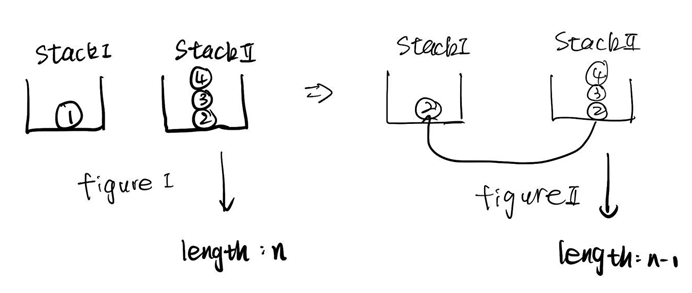
\includegraphics[width=16cm]{fig_ex3.png}
			\caption{Figure for exercise 3.}
			\label{fig_ex3}
		\end{figure}
	\end{solution}



	% 第四大题
	\question
	\begin{solution}
		Please refer to the code bundle.
	\end{solution}
\end{questions}
\end{document}